\documentclass[11pt,aspectratio=169]{beamer}
%%%%%%%%% GENERAL PACKAGES
%\usepackage[dvipsnames]{xcolor}
%\usepackage{pdfpages}
%\usetheme[progressbar=frametitle]{metropolis}
%\setbeamercolor{background canvas}{bg=white}
%\usepackage{appendixnumberbeamer}
%\usepackage{booktabs}
%\usepackage[scale=2]{ccicons}
%\usepackage{pgfplots}
%\usepgfplotslibrary{dateplot}
%\usepackage{xspace}
%\newcommand{\themename}{\textbf{\textsc{metropolis}}\xspace}
%\usepackage[absolute,overlay]{textpos}






%%%%%%%%% COLOR THEME

% Define some colors:
\definecolor{DarkFern}{HTML}{407428}
\definecolor{DarkCharcoal}{HTML}{4D4944}
\definecolor{AlertColor}{RGB}{89,124,158}
\definecolor{HighLight}{RGB}{96,95,134}
\definecolor{Important}{RGB}{234,122,133}
\definecolor{Yellow}{HTML}{00539C}
\colorlet{Fern}{DarkFern!85!white}
\colorlet{Charcoal}{DarkCharcoal!85!white}
\colorlet{LightCharcoal}{Charcoal!50!white}
\colorlet{HighLight2}{AlertColor}
\colorlet{DarkRed}{red!70!black}
\colorlet{DarkBlue}{blue!70!black}
\colorlet{DarkGreen}{green!70!black}
\definecolor{RoyalBlue}{HTML}{00539C}
\definecolor{Peach}{HTML}{EEA47F}
\definecolor{ForestGreen}{HTML}{2C5F2D}
\definecolor{MossGreen}{HTML}{E8FCC9}
\definecolor{SeaGreen}{HTML}{2E8B57}
% Use the colors:
\setbeamercolor{title}{fg=Fern}
\setbeamercolor{frametitle}{fg=MossGreen,bg=ForestGreen}
\setbeamercolor{normal text}{fg=Charcoal!70!black}
\setbeamercolor{block title}{fg=black,bg=Fern!25!white}
\setbeamercolor{block body}{fg=black,bg=Fern!10!white}
\setbeamercolor{block title alerted}{fg=black,bg=DarkRed!25!white}
\setbeamercolor{block body alerted}{fg=black,bg=DarkRed!10!white}
\setbeamercolor{alerted text}{fg=DarkRed}
\setbeamercolor{itemize item}{fg=Charcoal}



%%%%%%%%% OTHER COMMANDS
\newcommand{\indep}{\perp\!\!\! \perp}
\newcommand{\comment}[1]{}
\newcommand{\bs}{\boldsymbol}
\newcommand{\tr}{\text{trace}}
\newcommand{\sgn}{{\rm sgn}}
\def\T{\top}
%\newcommand{\det}{\text{det}}
\newcommand{\var}{\mathrm{var}}
\newcommand{\cC}{{\cal C}}
\renewcommand{\d}{{\rm d}}
\newcommand{\cG}{{\cal G}}
\newcommand{\cV}{{\cal V}}
\newcommand{\cE}{{\cal E}}
\newcommand{\cM}{{\cal M}}
\newcommand{\cP}{{\cal P}}
\newcommand{\cX}{{\cal X}}
\newcommand{\cY}{{\cal Y}}
\newcommand{\X}{\mathbf{X}}
\newcommand{\Y}{\mathbf{Y}}
\newcommand{\x}{\mathbf{x}}
\newcommand{\y}{\mathbf{y}}
\newcommand{\z}{\mathbf{z}}

\newcommand{\argmin}{\operatornamewithlimits{argmin}}
\newcommand{\eps}{\varepsilon}
\newcommand{\<}{\langle}
\renewcommand{\>}{\rangle}


%

\setbeamertemplate{navigation symbols}{}
\setbeamertemplate{footline}[text line]{%
    \hfill\strut{%
        \scriptsize\sf\color{black!60}%
        \quad\insertframenumber/\inserttotalframenumber
    }
    %\hfill
    }


\usenavigationsymbolstemplate{}
\setbeamersize{text margin left=.2cm,text margin right=.2cm} 
\addtobeamertemplate{frametitle}{}{\vspace{-1.2mm}}
\setbeamertemplate{itemize item}{$\bullet$}

\setbeamertemplate{itemize subitem}{\tiny\raise1.5pt\hbox{\donotcoloroutermaths$\blacktriangleright$}}
\setbeamertemplate{itemize subsubitem}{\tiny\raise1.5pt\hbox{\donotcoloroutermaths$\blacktriangleright$}}
\setbeamertemplate{enumerate item}{\insertenumlabel.}
\setbeamertemplate{enumerate subitem}{\insertenumlabel.\insertsubenumlabel}
\setbeamertemplate{enumerate subsubitem}{\insertenumlabel.\insertsubenumlabel.\insertsubsubenumlabel}
\setbeamertemplate{enumerate mini template}{\insertenumlabel}






\newcommand{\TODO}[1]{{\color{red}{[TODO: #1]}}}


\newcommand{\R}{\mathbb R}
\newcommand{\E}{\mathbb E}
\renewcommand{\P}{\mathbb P}


\DeclareMathOperator*{\cov}{cov}


\newsavebox{\zerobox}
\newenvironment{nospace}
{\par\edef\theprevdepth{\the\prevdepth}\nointerlineskip
  \setbox\zerobox=\vtop to 0pt\bgroup
  \hrule height0pt\kern\dimexpr\baselineskip-\topskip\relax
}
{\par\vss\egroup\ht\zerobox=0pt \wd\zerobox=0pt \dp\zerobox=0pt
  \box\zerobox}

\usepackage{soul}
\makeatletter
\let\HL\hl
\renewcommand\hl{%
  \let\set@color\beamerorig@set@color
  \let\reset@color\beamerorig@reset@color
  \HL}
  \makeatother

\usepackage[absolute,overlay]{textpos}

\newcommand{\source}[1]{\begin{textblock*}{4cm}(8.7cm,8.6cm)
    \begin{beamercolorbox}[ht=0.5cm,right]{framesource}
        \usebeamerfont{framesource}\usebeamercolor[fg]{framesource} Source: {#1}
    \end{beamercolorbox}
\end{textblock*}}

%\usecolortheme{whale}

\title[Calculus and Linear Algebra]{Lecture 2 : Calculus and Linear Algebra}
\author[Piotr Zwiernik, Barcelona School of Economics]{Piotr Zwiernik \\ $\;$\\
Mathematics Brush-up\\ $\;$\\ $\;$\\

\includegraphics[width=1.5in]{img/bse.png}  
}
\date{}

%\beamerdefaultoverlayspecification{<+->}

\begin{document}
\begin{frame}
\titlepage
\end{frame}

%========================================================
%                  INTEGRATION
%========================================================

\begin{frame}{Chapter 4: Integration}
Often a function $f$ is given and we are looking for \hl{$F$ whose derivative is $f$}.
\bigskip

\textcolor{SeaGreen}{Example:} the marginal cost function $C'(x)$ is known (how cost changes with production $x$). We want the cost $C(x)$ itself.
\bigskip

\textcolor{SeaGreen}{Idea:} \textbf{integration} reverses differentiation: it accumulates small changes.
\bigskip

\textcolor{SeaGreen}{Read} Chapter 5 of Werner-Sotskov \quad
\textcolor{SeaGreen}{Exercises} 5.1(a)-(b), 5.2(a)-(b), 5.3(c)
\end{frame}

\begin{frame}{Indefinite integrals}
A differentiable $F$ is an \textcolor{SeaGreen}{antiderivative} of $f$ if $F'(x)=f(x)$ on a common domain.
\bigskip

\textcolor{SeaGreen}{Fact:} all antiderivatives differ by a constant: if $F'(x)=f(x)$, then any $\tilde F(x)=F(x)+c$ also satisfies $\tilde F'(x)=f(x)$.
\bigskip

\textcolor{SeaGreen}{Definition:} the \textcolor{SeaGreen}{indefinite integral} is
\[
\int f(x)\,dx \;=\; F(x)+c.
\]
\textcolor{SeaGreen}{Linearity:}
\begin{enumerate}
\item $\int (f+g)\,dx=\int f\,dx+\int g\,dx$
\item $\int c\,f\,dx=c\int f\,dx$
\end{enumerate}
\end{frame}

\begin{frame}{Indefinite integrals you should know}
\textcolor{SeaGreen}{Templates:}
\begin{enumerate}
\item $\displaystyle \int x^n\,dx=\frac{x^{n+1}}{n+1}+c$, $n\neq -1$ \quad 
\item $\displaystyle \int \frac{1}{x}\,dx=\log|x|+c$
\item $\displaystyle \int e^x\,dx=e^x+c$
\item $\displaystyle \int \sin x\,dx=-\cos x+c$
\item $\displaystyle \int \cos x\,dx=\sin x+c$
\item $\displaystyle \int a^x\,dx=\frac{a^x}{\log a}+c \quad (a>0,a\neq 1)$
\end{enumerate}
{\small Always check by differentiating the right-hand side.}
\end{frame}

\begin{frame}{Integration by substitution}
\begin{block}{Theorem (Substitution)}
If $t=g(x)$ and $F$ is an antiderivative of $f$, then
\[
\int f(g(x))\,g'(x)\,dx=\int f(t)\,dt=F(t)+c=F(g(x))+c.
\]
\end{block}
\textcolor{SeaGreen}{Examples:}
\[
1.\ \int (ax+b)^n\,dx
= \frac{1}{a}\int t^n\,dt
= \frac{(ax+b)^{n+1}}{a(n+1)}+c.
\]
{\tiny ($t=ax+b$, so $dt=a\,dx$.)}
\[
2.\ \int \frac{e^x}{\sqrt[3]{1+e^x}}\,dx
= \int t^{-1/3}\,dt
= \frac{3}{2}t^{2/3}+c
= \frac{3}{2}(1+e^x)^{2/3}+c.
\]
{\tiny ($t=1+e^x$, so $dt=e^x\,dx$.)}
\end{frame}

\begin{frame}{Integration by parts}
\begin{block}{Theorem (Integration by parts)}
For differentiable $u,v$,
\[
\int u(x)v'(x)\,dx = u(x)v(x) - \int u'(x)v(x)\,dx.
\]
{\tiny Proof: Differentiate $u(x)v(x)$ and integrate.}
\end{block}
\textcolor{SeaGreen}{Example:} with $u=\log x$, $v'=1$,
\[
\int \log x\,dx = x\log x - \int 1\,dx = x(\log x-1)+c.
\]
\end{frame}

\begin{frame}{A combo: substitution then parts}
Compute $\int \sin\sqrt{x}\,dx$.
\bigskip

Substitute $t=\sqrt{x}$, so $x=t^2$ and $dx=2t\,dt$:
\[
\int \sin\sqrt{x}\,dx=2\int t\sin t\,dt.
\]
Now parts with $u=t$, $v'=\sin t$:
\[
2\int t\sin t\,dt
=2\Big(-t\cos t+\int \cos t\,dt\Big)
=2(-t\cos t+\sin t)+c.
\]
Back-substitute $t=\sqrt{x}$:
\[
\boxed{\ \int \sin\sqrt{x}\,dx=2\big(-\sqrt{x}\cos\sqrt{x}+\sin\sqrt{x}\big)+c\ }.
\]
\end{frame}


\begin{frame}[plain]{}
	\centering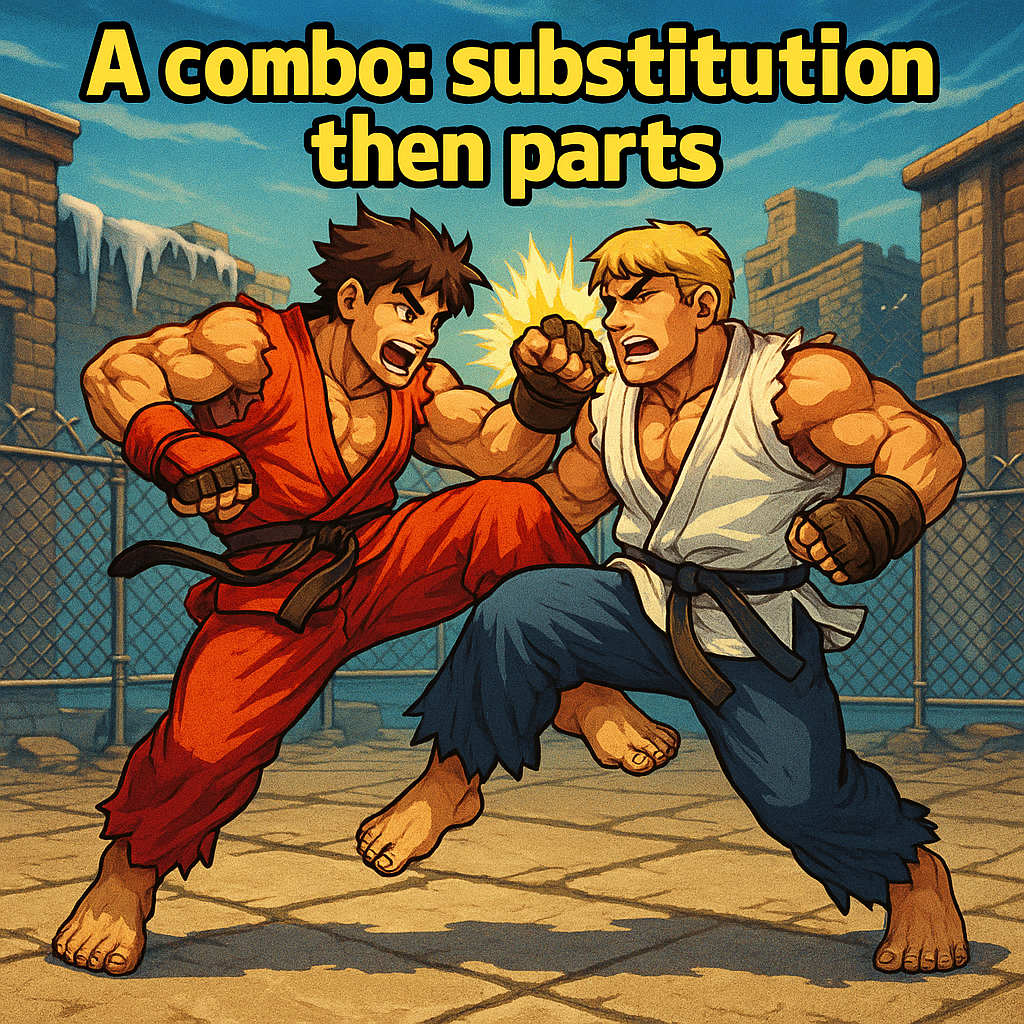
\includegraphics[scale=.25]{vbreaks/combo}
\end{frame}





\begin{frame}{Definite integral as area and accumulation}
For continuous $f:[a,b]\to\mathbb{R}$ with $f\ge 0$, the \textcolor{SeaGreen}{definite integral}
\[
\int_a^b f(x)\,dx
\]
is the area under $f$ between $a$ and $b$. More generally it accumulates signed change.
\bigskip

\textcolor{SeaGreen}{Properties:}
\begin{enumerate}
\item $\int_b^a f=-\int_a^b f$
\item $\int_a^b c f=c\int_a^b f$
\item If $c\in[a,b]$, then $\int_a^b f=\int_a^c f+\int_c^b f$
\item $\Big|\int_a^b f\Big|\le \int_a^b |f|$
\item If $f\le g$ on $[a,b]$, then $\int_a^b f\le \int_a^b g$
\end{enumerate}

\bigskip
\textcolor{SeaGreen}{Some uses:} cumulative revenue from a known marginal revenue curve, energy used by a device with power draw $P(t)$, or probability mass from a density.
\end{frame}

\begin{frame}[label=ftc]{Fundamental Theorem of Calculus}
\begin{alertblock}{Fundamental Theorem of Calculus}
If $f$ is continuous on $[a,b]$ and $F$ is an antiderivative of $f$, then
\[
\int_a^b f(x)\,dx = F(b)-F(a).
\]
Moreover, $G(t)=\int_a^t f(x)\,dx$ is differentiable and $G'(t)=f(t)$.
\end{alertblock}

\textcolor{SeaGreen}{Marginal to total:} If $C'(x)$ is marginal cost, then the change in total cost from $x=300$ to $x=400$ is
\[
C(400)-C(300)=\int_{300}^{400} C'(x)\,dx.
\]

\textcolor{SeaGreen}{Example:} $C'(x)=6-\dfrac{60}{x+1}$ for $x\in[0,1000]$:
\[
\int_{300}^{400}\!\! \Big(6-\frac{60}{x+1}\Big) dx
=\Big(6x-60\log|x+1|\Big)_{300}^{400}\approx 582.79.
\]
\end{frame}



\begin{frame}{Application: proving $e=\lim_{n\to\infty}(1+\tfrac1n)^n$ via integrals}
\ \\[-1mm]
Define $\displaystyle \log x=\int_1^x \frac{1}{t}\,dt$. Let $e^x$ be the inverse of $\log x$; then $1=\int_1^e \frac{1}{t}\,dt$.
\bigskip

For $t\in[1,1+\frac{1}{n}]$,
\[
\frac{1}{n+1}=\int_1^{1+\frac{1}{n}}\frac{1}{1+\frac{1}{n}}\,dt
\le \int_1^{1+\frac{1}{n}}\frac{1}{t}\,dt
\le \int_1^{1+\frac{1}{n}}1\,dt=\frac{1}{n}.
\]
So
\[
\frac{1}{n+1}\le \log\Big(1+\frac{1}{n}\Big)\le \frac{1}{n}.
\]
Exponentiate and rearrange to obtain
$$ 
\frac{e}{1+\frac{1}{n}}\le \Big(1+\frac{1}{n}\Big)^n \le e, 
$$
and let $n\to\infty$.

\hfill
\includegraphics[width=1cm]{img/qed.jpg}
\end{frame}

\begin{frame}{Application: Taylor with integral remainder (up to $n=2$)}
Apply FTC repeatedly:
\begin{align*}
f(x)
&= f(x_0)+\int_{x_0}^x f'(t_1)\,dt_1 \\
&= f(x_0)+f'(x_0)(x-x_0)+\int_{x_0}^x\!\int_{x_0}^{t_1} f''(t_2)\,dt_2\,dt_1 \\
&= f(x_0)+f'(x_0)(x-x_0)+\frac{f''(x_0)}{2}(x-x_0)^2
+ \int_{x_0}^x\!\int_{x_0}^{t_1}\!\int_{x_0}^{t_2} f^{(3)}(t_3)\,dt_3\,dt_2\,dt_1.
\end{align*}
By the intermediate value theorem there is $y$ between $x_0$ and $x$ with
\[
\int\!\!\int\!\!\int f^{(3)}(t_3)\,dt_3\,dt_2\,dt_1
= \frac{f^{(3)}(y)}{3!}(x-x_0)^3.
\]
\end{frame}

%========================================================
%                  VECTORS
%========================================================

\begin{frame}{Chapter 5: Vectors}
A \textcolor{SeaGreen}{vector} is an ordered $n$-tuple of real numbers: $\bs v=(v_1,\ldots,v_n)\in\mathbb{R}^n$.
\bigskip

\textcolor{SeaGreen}{Why care in econ/data:}
\begin{itemize}
\item a bundle of $n$ goods (quantities),
\item a user's features or a product's attributes,
\item a portfolio's weights across $n$ assets,
\item a document's word counts or an embedding.
\end{itemize}
\bigskip

\textcolor{SeaGreen}{Read} Chapter 6 of Werner-Sotskov; Simon-Blume Chs. 10-11. 
\bigskip

\textcolor{SeaGreen}{Exercises} 6.2, 6.3, 6.4, 6.6, 6.7, 6.8
\end{frame}

\begin{frame}{Definition and notation}
A \textcolor{SeaGreen}{vector} ${\bf v}$ is an ordered $n$-tuple $(v_1,\dots,v_n)$ of real numbers called \textcolor{SeaGreen}{coordinates}.
\bigskip

\textcolor{SeaGreen}{Notation:} $\bs v=(v_1,\ldots,v_n)\in\mathbb{R}^n$.\\ \quad\quad\quad\;\quad The zero vector is $\bs 0=(0,\ldots,0)$.\\ 
\quad\quad\quad\;\quad The $i$-th unit vector is $\bs e_i$ (a 1 in position $i$, zeros elsewhere).
\bigskip

\textcolor{SeaGreen}{Operations:}
\[
\bs u+\bs v=(u_1+v_1,\ldots,u_n+v_n),\quad
\lambda\bs v=(\lambda v_1,\ldots,\lambda v_n).
\]
These satisfy the usual commutative, associative, and distributive laws.\\[4mm]
\end{frame}

\begin{frame}{Sum and difference of two vectors}
Note $\bs u-\bs v\;=\;\bs u+ (-1)\bs v$.
\begin{figure}
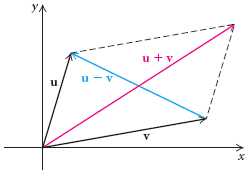
\includegraphics[width=2.5in]{img/sum}
\end{figure}
\end{frame}

\begin{frame}{Inner product and norm}
The \textcolor{SeaGreen}{inner product} (dot product) of $\bs u,\bs v\in\mathbb{R}^n$ is
\[
\langle \bs u,\bs v\rangle = \sum_{i=1}^n u_i v_i.
\]
The \textcolor{SeaGreen}{Euclidean norm} is $\|\bs v\|=\sqrt{\langle \bs v,\bs v\rangle}$.
\bigskip

\textcolor{SeaGreen}{Properties:}
\begin{enumerate}
\item $\langle \bs u,\bs v\rangle=\langle \bs v,\bs u\rangle$
\item $\langle \bs u,\bs v+\bs w\rangle=\langle \bs u,\bs v\rangle+\langle \bs u,\bs w\rangle$
\item \textcolor{SeaGreen}{Cauchy-Schwarz:} $|\langle \bs u,\bs v\rangle|\le \|\bs u\|\,\|\bs v\|$
\item \textcolor{SeaGreen}{Triangle inequality:} $\|\bs u+\bs v\|\le \|\bs u\|+\|\bs v\|$
\end{enumerate}
\medskip
\textcolor{blue}{Example (platform revenue):} hours watched per genre $\bs u=(500,200,50)$ and euro-per-hour rates $\bs v=(2,3,5)$ yield total revenue
$\langle \bs u,\bs v\rangle=2150$.
\end{frame}

\begin{frame}{The Law of Cosines and angles}
\[
\|\bs u-\bs v\|^2=\|\bs u\|^2+\|\bs v\|^2 - 2\|\bs u\|\,\|\bs v\|\cos(\angle(\bs u,\bs v)).
\]
Equivalently,
\[
\cos(\angle(\bs u,\bs v))=\frac{\langle \bs u,\bs v\rangle}{\|\bs u\|\,\|\bs v\|}.
\]
\begin{minipage}{9cm}
	\begin{small}
	We prove that $c^2=a^2+b^2-2ab \cos(C)$:\\[3mm]
By Pythagoras, $x^2+y^2=b^2$ and $(a-x)^2+y^2=c^2$. Subtract to eliminate $y^2$ to get $c^2=a^2+b^2-2a x$. Use $\cos C = x/b$.
\end{small}
\end{minipage}\begin{minipage}{5cm}
	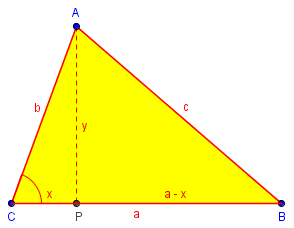
\includegraphics[width=2.5in]{img/cos}
\end{minipage}
\end{frame}

\begin{frame}{Orthogonality}
\textcolor{SeaGreen}{Definition:} $\bs u\perp \bs v$ if $\langle \bs u,\bs v\rangle=0$.
\bigskip

\textcolor{SeaGreen}{Angle example:} For $\bs u=(2,-1,3)$ and $\bs v=(5,-4,-1)$,
\[
\langle \bs u,\bs v\rangle=11,\quad
\cos\angle(\bs u,\bs v)=\frac{11}{\sqrt{14}\sqrt{42}}\approx 0.4537,
\]
so the angle is about $63^\circ$.
\bigskip

\textcolor{SeaGreen}{Geometric test:} $\bs u\perp \bs v$ iff $\|\bs u-\bs v\|^2=\|\bs u\|^2+\|\bs v\|^2$.
\end{frame}

\begin{frame}{Cauchy-Schwarz via completing the square}
Assume nonzero $\bs u,\bs v$. For any real $t$,
\[
0\le \|\bs u-t\bs v\|^2=\|\bs u\|^2-2t\,\langle \bs u,\bs v\rangle+t^2\|\bs v\|^2.
\]
Complete the square in $t$:
\[
\|\bs u\|^2-2t\,\langle \bs u,\bs v\rangle+t^2\|\bs v\|^2
=\|\bs v\|^2\!\left(t-\frac{\langle \bs u,\bs v\rangle}{\|\bs v\|^2}\right)^{\!2}
+\Big(\,\|\bs u\|^2-\frac{\langle \bs u,\bs v\rangle^2}{\|\bs v\|^2}\Big).
\]
Since the left side is $\ge 0$ for all $t$, the second term must be $\ge 0$:
\[
\langle \bs u,\bs v\rangle^2\le \|\bs u\|^2\,\|\bs v\|^2.
\]
\textcolor{SeaGreen}{Equality condition:} equality holds iff $\|\bs u-t\bs v\|^2=0$ for $t=\frac{\langle \bs u,\bs v\rangle}{\|\bs v\|^2}$, i.e., $\bs u=t\,\bs v$ (collinear vectors).

\hfill
\includegraphics[width=1cm]{img/qed.jpg}
\end{frame}



\begin{frame}{Linear dependence, independence, and bases}
\textcolor{SeaGreen}{Linear combination:} $\bs u=\sum_{i=1}^m \lambda_i \bs v_i$.
\bigskip

\textcolor{SeaGreen}{Linear independence:} $\{\bs v_1,\ldots,\bs v_m\}$ is linearly independent if
\[
\sum_{i=1}^m \lambda_i \bs v_i=\bs 0 \quad\Rightarrow\quad \lambda_1=\cdots=\lambda_m=0.
\]
\textcolor{SeaGreen}{Basis:} Any $n$ linearly independent vectors in $\mathbb{R}^n$ form a basis. Then every $\bs u\in\mathbb{R}^n$ has a \alert{unique} representation $\bs u=\sum_{i=1}^n \lambda_i \bs v_i$.
\bigskip

\textcolor{SeaGreen}{Standard basis:} $\{\bs e_1,\ldots,\bs e_n\}$.
\end{frame}

\begin{frame}{Subspaces, span, and dimension}
For $E=\{\bs v_1,\ldots,\bs v_k\}$, the \textcolor{SeaGreen}{span} is
\[
\mathrm{span}(E)=\Big\{\sum_{i=1}^k \lambda_i \bs v_i:\ \lambda_i\in\mathbb{R}\Big\}.
\]
A \textcolor{SeaGreen}{subspace} $V\subset\mathbb{R}^n$ is any span. A \textcolor{SeaGreen}{basis of $V$} is a linearly independent set that spans $V$.
The \textcolor{SeaGreen}{dimension} of $V$ is the size of any basis.
\bigskip

\textcolor{SeaGreen}{Exercise:} Basis of $V=\{(x_1,x_2,x_3)\in\mathbb{R}^3:\ x_1+x_2+x_3=0\}$.
\end{frame}



\begin{frame}[label=orthogonal]{Orthogonal complement and projection}
\begin{block}{Orthogonal complement}
For a subspace $V\subset\mathbb{R}^n$,
\[
V^\perp=\{\bs x:\ \langle \bs x,\bs v\rangle=0\ \forall \bs v\in V\}.
\]
\end{block}
\begin{alertblock}{Projection theorem}
For any $\bs y\in\mathbb{R}^n$ and subspace $V$, there is a unique $\hat{\bs y}\in V$ with $\bs y-\hat{\bs y}\in V^\perp$. We call $\hat{\bs y}$ the orthogonal projection of $\bs y$ onto $V$.
\end{alertblock}

\textcolor{SeaGreen}{Least squares view:} With design matrix $\bs X\in\mathbb{R}^{n\times d}$ and response $\bs y$, the LS fit $\hat{\bs y}$ is the projection of $\bs y$ onto the column space of $\bs X$.
\[
\hat{\bs y}=\bs X(\bs X^\top\bs X)^{-1}\bs X^\top\bs y.
\]
\end{frame}


\begin{frame}{}
\centering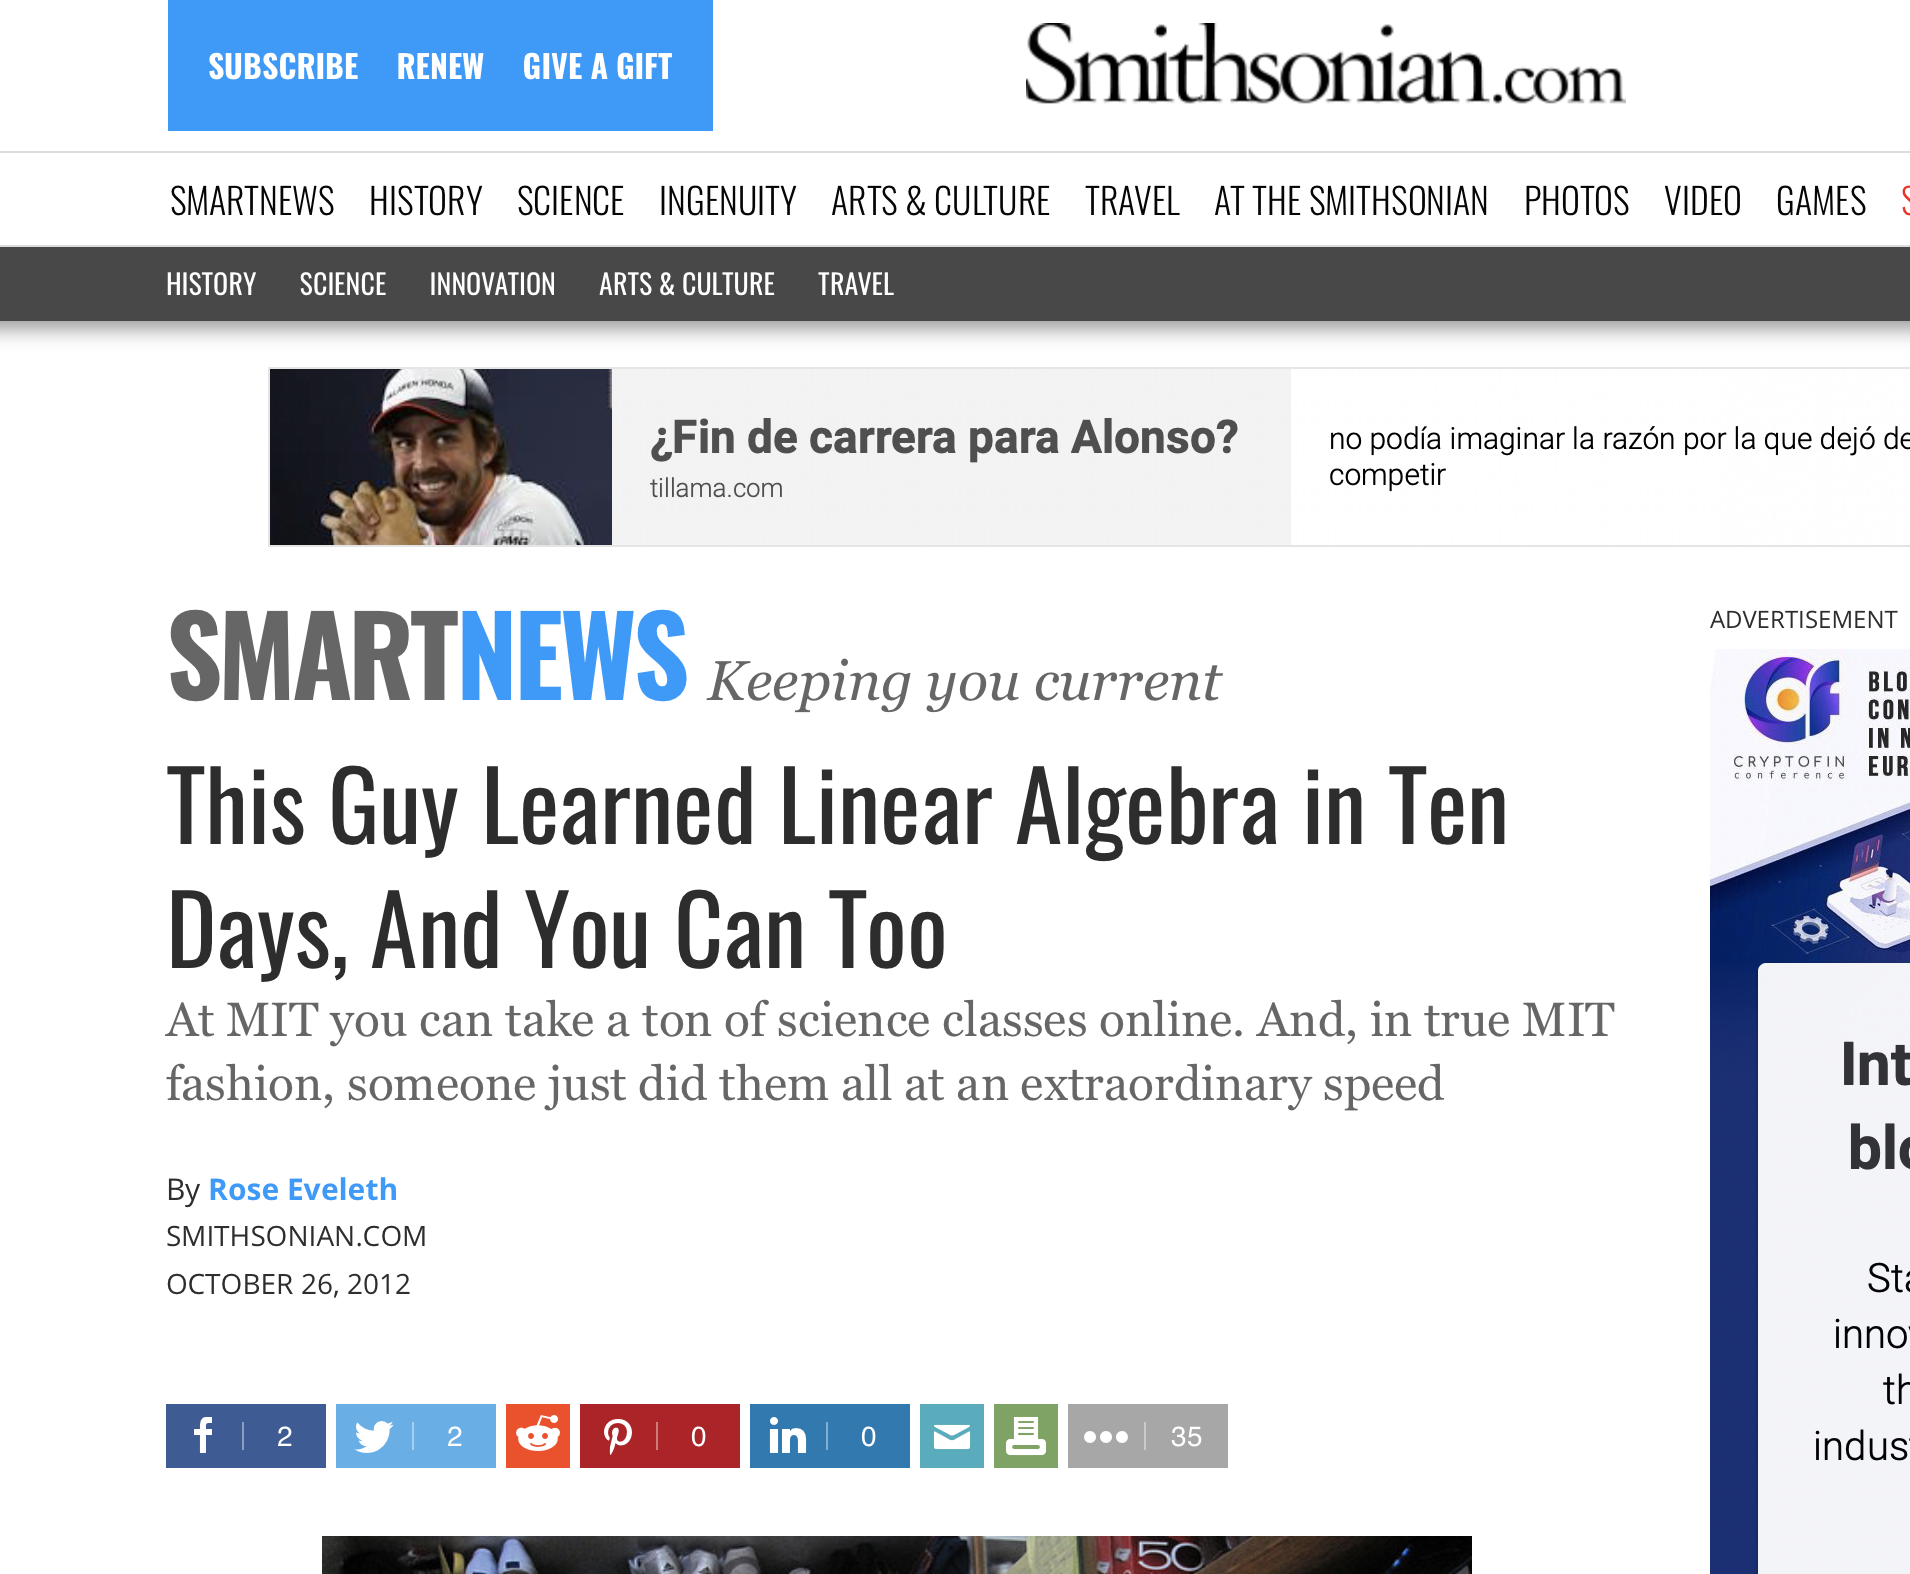
\includegraphics[height=\paperheight]{img/LinAlg10days.png}	
\end{frame}

%========================================================
%                  MATRICES
%========================================================

\begin{frame}{Chapter 6: Matrices and determinants}
A \textcolor{SeaGreen}{matrix} $A\in\mathbb{R}^{m\times n}$ is a table with $m$ rows, $n$ columns. The $(i,j)$ entry is $a_{ij}$.
\bigskip

We recall basic facts about matrices.
\bigskip

\textcolor{SeaGreen}{Why care:} matrices express linear maps, data tables, network flows, input-output models, regressions, transformations, and more.
\bigskip

\textcolor{SeaGreen}{Read} Werner-Sotskov Ch. 7; Simon-Blume Chs. 8-9. \\[4mm]
\textcolor{SeaGreen}{Exercises} 7.6, 7.9(b,c,d), 7.12, 7.14(a), 7.16, 7.18
\end{frame}



\begin{frame}{Matrices}
	A table of numbers with $m$ rows and $n$ columns: $A\in \R^{m\times n}$. The $(i,j)$-th entry is denoted by $a_{ij}$.\\[.3cm]
	Special matrices: 
\begin{itemize}
	\item zero matrix: $\bs 0_{m\times n}\in \R^{m\times n}$\\[.2cm]
	\item identity matrix: $\mathbb I_n\in \R^{n\times n}$.\\[.2cm]
		\item \textcolor{SeaGreen}{transposition}: $A^T\in \R^{n\times m}$, $(A^T)_{ij}=a_{ji}$.\\[.2cm]
		\item square matrix: $m=n$.\\[.2cm]
		\item symmetric matrix: square matrix such that $A=A^T$.\\[.2cm]
		\item diagonal matrix: $a_{ij}=0$ if $i\neq j$.\\[.2cm]
		\item lower (upper) trianglar: $a_{ij}=0$ if $i<j$ ($i>j$).\\[.2cm]
		\item $\bs v\in \R^n$ is treated as $n\times 1$ matrix, $\R^n\simeq \R^{n\times 1}$. 
\end{itemize}	
\end{frame}




\begin{frame}{Basic matrix operations}
Addition and scalar multiplication are entrywise:
\[
(A+B)_{ij}=a_{ij}+b_{ij},\qquad (\lambda A)_{ij}=\lambda a_{ij}.
\]
They satisfy the usual commutative, associative, and distributive laws.
\bigskip

\textcolor{SeaGreen}{Matrix product:} If $A\in\mathbb{R}^{m\times p}$ and $B\in\mathbb{R}^{p\times n}$, then $C=AB\in\mathbb{R}^{m\times n}$ with
\[
c_{ij}=\sum_{k=1}^p a_{ik}b_{kj}.
\]
\textcolor{SeaGreen}{Example:}
\[
\begin{pmatrix}2& 3 & 4 & 1\\
7 & -1 & 0 & 4
\end{pmatrix} 
\begin{pmatrix}2& 7\\
3 & -1 \\
4 & 0 \\
1& 4
\end{pmatrix}
=
\begin{pmatrix}30&  15\\
15 & 66
\end{pmatrix}.
\]
\end{frame}

\begin{frame}{Algebraic properties}
\textcolor{SeaGreen}{Facts:}
\begin{enumerate}
\item $(AB)C=A(BC)$
\item $A(B+C)=AB+AC$ and $(A+B)C=AC+BC$
\item Generally \textbf{not} commutative: $AB\neq BA$
\item $AI_n=I_mA=A$ (dimensions must match)
\item $(A^T)^T=A$, $(A+B)^T=A^T+B^T$, $(\lambda A)^T=\lambda A^T$, $(AB)^T=B^T A^T$
\end{enumerate}
\textcolor{SeaGreen}{Remark:} $AA^T$ is always symmetric.
\end{frame}

\begin{frame}{Matrix times vector}
We treat $\mathbb{R}^n$ as column vectors $\mathbb{R}^{n\times 1}$. If $A\in\mathbb{R}^{m\times n}$ and $\bs x\in\mathbb{R}^n$ then $A\bs x\in\mathbb{R}^m$ is a linear combination of the columns of $A$ with coefficients $x_i$:
\[
A\bs x = x_1\bs a_1+\cdots+x_n\bs a_n.
\]
\bigskip

e.g. \textbf{Another look at the LS method}: $\bs X\in \R^{n\times d}$, $\bs y\in \R^n$
$$
{\rm minimize}_{\beta\in \R^d}\quad \|\bs y-\bs X\beta\|^2
$$
Finds the closest point to $\bs y$ in the space spanned by the columns of $\bs X$.
\end{frame}

\begin{frame}[label=orthogonal2]{Orthogonal projection}
		\textbf{Theorem: }Given a vector $\bs y\in \R^n$ and a subspace $V\subset \R^n$ there exists a unique $\hat{\bs y}\in V$ such that \;\;$\bs y-\hat{\bs y}\in V^\perp$.
	Let $\bs x_1,\ldots,\bs x_d$ be a basis of $V\subset \R^n$.\\[.3cm]
	$\bs X\in \R^{n\times d}$ with columns  $\bs x_1,\ldots,\bs x_d$.\\[.5cm]
	$\hat{\bs y}\in V$ means \quad $\hat{\bs y}=\bs X\bs \lambda$\quad  for some $\bs \lambda=(\lambda_1,\ldots,\lambda_d)$.\\[.3cm]
	$\bs y-\hat{\bs y}\in V^\perp$ \quad means \quad $\bs X^\top(\bs y-\hat{\bs y})=\bs 0$.\\[.5cm]
	The unique solution: \quad $\bs \lambda=(\bs X^\top \bs X)^{-1}\bs X^\top\bs y$.
\end{frame}


\begin{frame}{Matrix inverse}
A square matrix $A$ is \textcolor{SeaGreen}{invertible} if there exists a matrix $A^{-1}$ such that
$$
A A^{-1}=A^{-1}A=I.
$$
	We want to show:
		\begin{beamercolorbox}[wd=\paperwidth,sep=0pt]{important}	
		\begin{center}
$A\in \R^{n\times n}$ is invertible \quad $\Longleftrightarrow$\quad $A\bs x=\bs 0_n$ only for $\bs x= \bs 0_n$.		
		\end{center}
\end{beamercolorbox}
Two observations:
\begin{enumerate}
	\item $A\bs x=\bs 0$ only for $\bs x=\bs 0$\quad iff\quad columns of $A$ are lin. independent.
	\item $n$ independent vectors in $\R^n$ form a basis and so $\forall i=1,\ldots, n$ $\exists \bs b_i$ such that $A\bs b_i=\bs e_i$.
	\item This gives $B\in \R^{n\times n}$ such that $AB=\mathbb I_n$.
%	\item $AB=\mathbb I_n$ means $A\bs b_i=\bs e_i$ for $i=1,\ldots, n$ and so the columns of $A$ form a basis of $\R^n$. 
\end{enumerate}
\bigskip

This is enough to show that the matrix $\bs X^\top\bs X$ on slide~\ref{orthogonal2} is invertible.\\
\quad {\footnotesize Note: If $(\bs X^\top \bs X)\bs x=\bs 0$ then $\bs x^\top(\bs X^\top \bs X)\bs x=\bs 0$ but this only possible if $\bs x=\bs 0$.} 
\end{frame}




\begin{frame}{Important spaces and rank}
For $A\in\mathbb{R}^{m\times n}$:
\begin{itemize}
\item \textcolor{SeaGreen}{Column space} (image) $\mathrm{Im}(A)=\{A\bs x:\bs x\in\mathbb{R}^n\}\subset\mathbb{R}^m$
\item \textcolor{SeaGreen}{Row space} $\mathrm{Im}(A^T)\subset\mathbb{R}^n$
\item \textcolor{SeaGreen}{Kernel} (null space) $\ker(A)=\{\bs x:\ A\bs x=\bs 0\}\subset\mathbb{R}^n$
\item \textcolor{SeaGreen}{Rank} $\mathrm{rank}(A)=\dim \mathrm{Im}(A)=\dim \mathrm{Im}(A^T)$
\end{itemize}
\textcolor{SeaGreen}{Orthogonality:} Row space is orthogonal to $\ker(A)$.
\bigskip

\textcolor{SeaGreen}{Rank-nullity:} $\mathrm{rank}(A)+\dim\ker(A)=n$.
\bigskip

\textcolor{SeaGreen}{Try:} $A=\begin{bmatrix}1&0&2\\[2pt]0&1&1\end{bmatrix}$.
\end{frame}


\begin{frame}[plain,noframenumbering]{}
\begin{textblock*}{4cm}(5cm,1cm)
	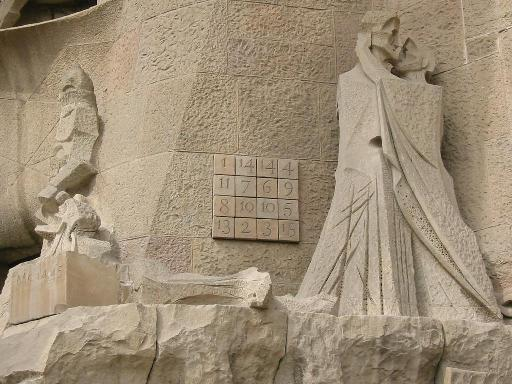
\includegraphics[scale=.5]{vbreaks/sf1}
\end{textblock*}
	\begin{textblock*}{4cm}(2cm,4.2cm)
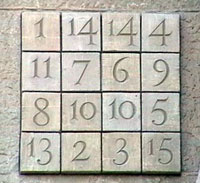
\includegraphics[scale=.7]{vbreaks/sf2}
	\end{textblock*}	
\end{frame}



\begin{frame}{Orthogonal matrices}
An $n \times n$ matrix $A$ is called \textcolor{SeaGreen}{orthogonal} if  $AA^\top=I_n$.
\vskip 12pt
\textcolor{SeaGreen}{Remark:} If $A$ is orthogonal, its row vectors (and also its column vectors) are pairwise orthogonal unit vectors.

\begin{small}Proof: Let $\bs r_i$ and $\bs r_j$ be the $i$-th and $j$-th rows of $A$.  
The $(i,j)$ entry of $AA^\top$ is the scalar product $\bs r_i^\top\bs r_j$.  
If $AA^\top=I$, then $\bs r_i^\top\bs r_j = 0$ for $i\neq j$ (orthogonality) and  
$\bs r_i^\top\bs r_i = \|\bs r_i\|^2 = 1$ (unit length).  
The same holds for columns using $A^\top A = I_n$.\end{small}
\vskip 12pt
\textcolor{SeaGreen}{Example:}
\begin{align*}
\begin{pmatrix}\tfrac{1}{\sqrt{2}}& \tfrac{1}{\sqrt{2}} \\
-\tfrac{1}{\sqrt{2}}& \tfrac{1}{\sqrt{2}}
\end{pmatrix}
\begin{pmatrix}
\tfrac{1}{\sqrt{2}}& -\tfrac{1}{\sqrt{2}}\\
\tfrac{1}{\sqrt{2}}& \tfrac{1}{\sqrt{2}}
\end{pmatrix}
=
\begin{pmatrix}1&  0\\
0 & 1
\end{pmatrix}
\end{align*}
\end{frame}



\begin{frame}{Elementary matrix operations}
Column or row operations:
\begin{enumerate}
\item \textcolor{SeaGreen}{Swap} two columns (or rows)
\item \textcolor{SeaGreen}{Scale} a column (or row) by $\lambda\neq 0$
\item \textcolor{SeaGreen}{Add} a multiple of one column (or row) to another
\end{enumerate}
Each is implemented by multiplying by a suitable elementary matrix on the right (for column ops) or left (for row ops). Useful for Gaussian elimination and determinant computation.

\begin{block}{}
	Let $A=\begin{bmatrix}
	a_{11} & a_{12}\\
	a_{21} & a_{22}
\end{bmatrix}$ and multiply from the right by $\begin{bmatrix}
	0 & 1\\
	1 & 0
\end{bmatrix}$, $\begin{bmatrix}
	\lambda & 0\\
	0 & 1
\end{bmatrix}$, or $\begin{bmatrix}
	1 & 0\\
	\lambda & 1
\end{bmatrix}$.
\end{block}

\end{frame}

%========================================================
%                  DETERMINANTS
%========================================================

\begin{frame}{Determinants: definition}
For $A\in\mathbb{R}^{n\times n}$, let $A_{ij}$ be the submatrix with row $i$ and column $j$ removed. Define recursively
\[
\det(A)=\sum_{j=1}^n (-1)^{1+j} a_{1j} \det(A_{1j}),\quad \det([a_{11}])=a_{11}.
\]
For $n=2$: $\det\begin{pmatrix}a&b\\ c&d\end{pmatrix}=ad-bc$.
\bigskip

For $n=3$:
\[
\det(A)=a_{11}a_{22}a_{33}+a_{12}a_{23}a_{31}+a_{13}a_{21}a_{32}
- a_{11}a_{23}a_{32}-a_{12}a_{21}a_{33}-a_{13}a_{22}a_{31}.
\]
\end{frame}

\begin{frame}{A memory aid for $n=3$}
\begin{figure}
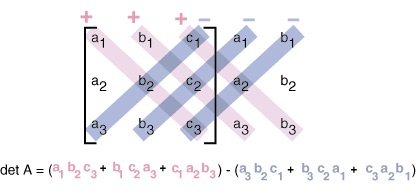
\includegraphics[width=4in]{img/deter} 
\end{figure}
\end{frame}

\begin{frame}{Cofactor expansion and properties}
\textcolor{SeaGreen}{Cofactor expansion:} expand by any row $i$ or any column $j$:
\[
\det(A)=\sum_{j=1}^n (-1)^{i+j} a_{ij}\det(A_{ij})
=\sum_{i=1}^n (-1)^{i+j} a_{ij}\det(A_{ij}).
\]
\textcolor{SeaGreen}{Properties:}
\begin{enumerate}
\item $\det(A)=\det(A^T)$
\item If $A$ is triangular, $\det(A)$ is the product of diagonal entries
\item $\det(AB)=\det(A)\det(B)$
\item Swapping two rows (or columns) flips the sign of $\det$
\item Scaling a row (or column) by $\lambda$ scales $\det$ by $\lambda$
\item Adding a multiple of one row to another leaves $\det$ unchanged
\item $\det(A)=0$ iff rows (or columns) are linearly dependent
\end{enumerate}
\end{frame}

\begin{frame}{Determinants by elimination}
Use row operations (keeping track of determinant changes) to reach triangular form.
\[
\begin{vmatrix}
1 & 2 & 0\\
3 & 0 & 1\\
1 & 2 & 3
\end{vmatrix}
\to
\begin{vmatrix}
1 & 2 & 0\\
0 & -6 & 1\\
1 & 2 & 3
\end{vmatrix}
\to
\begin{vmatrix}
1 & 2 & 0\\
0 & -6 & 1\\
0 & 0 & 3
\end{vmatrix}
= (-6)\cdot 3 = -18.
\]
{\tiny First: $r_2\leftarrow r_2-3r_1$. Then: $r_3\leftarrow r_3-r_1$.}
\bigskip

\textcolor{SeaGreen}{Geometric meaning:} $|\det(A)|$ is the area/volume scaling of the linear map $x\mapsto Ax$ (and its sign encodes orientation).
\end{frame}

%========================================================
%                  LINEAR SYSTEMS
%========================================================

\begin{frame}{Linear systems and Cramer's rule}
A system $A\bs x=\bs b$ with $A\in\mathbb{R}^{n\times n}$, unknown $\bs x\in\mathbb{R}^n$, and data $\bs b$.
If $A$ is \textcolor{SeaGreen}{nonsingular} ($\det A\neq 0$), the solution is unique.
\bigskip

\textcolor{SeaGreen}{Cramer's rule:} Let $A_j(\bs b)$ be $A$ with column $j$ replaced by $\bs b$. Then
\[
x_j=\frac{\det A_j(\bs b)}{\det A},\quad j=1,\ldots,n.
\]
\textcolor{SeaGreen}{Note:} Great for theory, not used for large-scale computation.
\bigskip

\textcolor{SeaGreen}{Example:}
\[
A=\begin{pmatrix}
2 & 3 & 5\\
1 & 0 & 2\\
-1 & -4 & 2
\end{pmatrix},\quad
\bs b=\begin{pmatrix}1\\7\\4\end{pmatrix}
\ \Rightarrow\
\bs x=\Big(\tfrac{75}{8},-\tfrac{63}{16},-\tfrac{19}{16}\Big).
\]
\end{frame}

%========================================================
%                  LINEAR MAPPINGS
%========================================================

\begin{frame}{Linear mappings}
A mapping $A:\mathbb{R}^n\to\mathbb{R}^m$ is \textcolor{SeaGreen}{linear} if
\[
A(\bs x_1+\bs x_2)=A(\bs x_1)+A(\bs x_2),\qquad
A(\lambda \bs x)=\lambda A(\bs x).
\]
Then there exists an $m\times n$ matrix (also denoted $A$) with $A(\bs x)=A\bs x$.
\bigskip

\textcolor{SeaGreen}{Columns as images:} $A(\bs e_i)=\bs a_i$ (the $i$-th column), and $A(\bs x)=\sum_i x_i A(\bs e_i)$.
\bigskip

\textcolor{SeaGreen}{Examples:} scalings, rotations, reflections, projections, feature maps in ML, Leontief input-output in economics.
\end{frame}

\begin{frame}{Two simple linear maps}
\begin{enumerate}
\item Reflection across the $y$-axis:
\[
A=\begin{pmatrix}-1&0\\ 0&1\end{pmatrix},\qquad
A\begin{pmatrix}x\\y\end{pmatrix}=\begin{pmatrix}-x\\y\end{pmatrix}.
\]
\item Rotation by $45^\circ$ counterclockwise:
\[
A=\begin{pmatrix}\tfrac{1}{\sqrt{2}}&-\tfrac{1}{\sqrt{2}}\\[2pt]
\tfrac{1}{\sqrt{2}}&\tfrac{1}{\sqrt{2}}\end{pmatrix}.
\]
Check the images of $\bs e_1$ and $\bs e_2$ to see the action.
\end{enumerate}
\end{frame}

%========================================================
%                  INVERSE MATRIX
%========================================================

\begin{frame}{Inverse matrix and properties}
A square $A$ is invertible if $A^{-1}$ exists with $AA^{-1}=A^{-1}A=I_n$.
\bigskip

\textcolor{SeaGreen}{Properties:}
\begin{enumerate}
\item $(A^{-1})^{-1}=A$
\item $(AB)^{-1}=B^{-1}A^{-1}$
\item $(A^T)^{-1}=(A^{-1})^T$
\item $(\lambda A)^{-1}=\lambda^{-1}A^{-1}$ for $\lambda\neq 0$
\item $\det(A^{-1})=1/\det(A)$
\end{enumerate}

\textcolor{SeaGreen}{Solve} $A\bs x=\bs b$ by $\bs x=A^{-1}\bs b$ when $A$ is invertible.
\end{frame}

\begin{frame}{Computing inverses}
\textcolor{SeaGreen}{Cofactor formula:} If $A$ is nonsingular,
\[
A^{-1}=\frac{1}{\det A}\,C(A)^T,\quad C(A)_{ij}=(-1)^{i+j}\det(A_{ij}).
\]
For $2\times 2$:
\[
\begin{pmatrix}a&b\\ c&d\end{pmatrix}^{-1}
=\frac{1}{ad-bc}\begin{pmatrix}d&-b\\ -c&a\end{pmatrix}.
\]
For larger $n$, numerical methods use elimination (LU), not cofactors.
\end{frame}

%========================================================
%                  INPUT-OUTPUT
%========================================================

\begin{frame}{Example: Input-output model}
Let $a_{ij}$ be units of good $i$ needed to produce 1 unit of good $j$. Put $A=(a_{ij})$.
Let $\bs x$ be total output and $\bs y$ the vector of final demand.
\bigskip

\textcolor{SeaGreen}{Accounting identity:} output = internal demand + final demand
\[
\bs x = A\bs x + \bs y
\quad\Leftrightarrow\quad
(I_n-A)\bs x=\bs y
\quad\Rightarrow\quad
\bs x=(I_n-A)^{-1}\bs y
\]
provided $I_n-A$ is invertible.
\bigskip

\textcolor{SeaGreen}{Interpretation:} $(I-A)^{-1}=I+A+A^2+\cdots$ accumulates direct, indirect, and higher-order input needs when it converges.
\end{frame}

\begin{frame}{A triangular example}
\textcolor{SeaGreen}{Theorem:} If $A$ is strictly upper triangular (zeros on and below diagonal), then $A^n=0$ and
\[
(I_n-A)^{-1}=I_n+A+A^2+\cdots+A^{n-1}.
\]
{\tiny Check $(I-A)(I+A+\cdots+A^{n-1})=I-A^n=I$.}
\bigskip

\textcolor{SeaGreen}{Example:}
\[
A=\begin{pmatrix}
0&3&5\\
0&0&2\\
0&0&0
\end{pmatrix},\quad
\bs y=\begin{pmatrix}1\\ 7\\ 4\end{pmatrix}
\ \Rightarrow\
\bs x=(66,15,4).
\]
\end{frame}

\end{document}